\section{Texture mapping}
\label{sec:tex}
\here{9}
A texture adds detail without geometry. A surface point gets coordinates $(u,v)$ (stored per vertex, or
computed from position), the texture is sampled there with filtering and mip-maps, and the result modulates a
material property. A procedural texture computes the value with a function instead of an image.
\begin{equation}
\text{bump: }\ \vect N'=\mathrm{normalize}\big(\vect N-\nabla h\big),\qquad
\text{mip level: }\ \lambda=\log_2\max\Big(\Big\lVert\tfrac{\partial(u,v)}{\partial x}\Big\rVert,\Big\lVert\tfrac{\partial(u,v)}{\partial y}\Big\rVert\Big)
\label{eq:tex}
\end{equation}

\begin{figure}[htbp]
\centering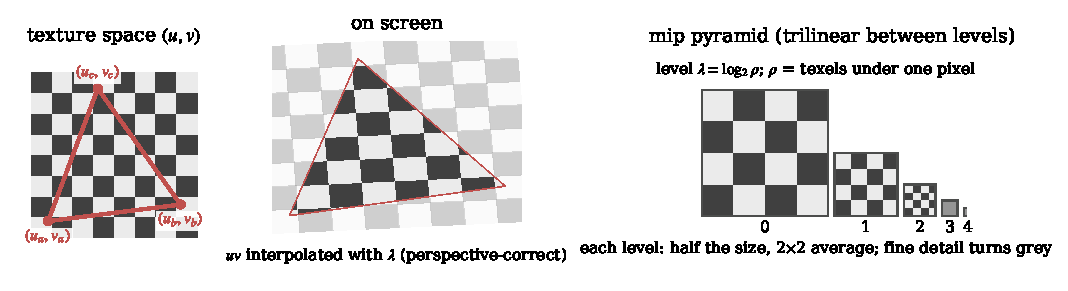
\includegraphics[width=\linewidth]{figures/diagrams/d_texture.pdf}
\caption{Texture mapping: each vertex carries $(u,v)$; inside the triangle $(u,v)$ is interpolated like any attribute and the texture is looked up there. Far away many texels fall under one pixel, so the lookup uses a smaller, pre-averaged mip level (Eq.~\ref{eq:tex}); fine detail fades to its average instead of shimmering.}
\label{fig:d-tex}
\end{figure}

\begin{figure}[htbp]
\centering
\begin{subfigure}{\linewidth}\img{figures/img/annot/tex_scene.jpg}{\linewidth}\caption{The SAM position: every surface
is either computed (procedural) or looked up in an image.}\end{subfigure}\\[1.2mm]
\begin{subfigure}{0.40\linewidth}\raw{lab/material_grid}{\linewidth}\caption{The procedural materials on spheres.}\end{subfigure}\hfill
\begin{subfigure}{0.58\linewidth}\raw{scene/m6_tree_close}{\linewidth}\caption{An imported tree: UV-mapped bark and
alpha-tested leaves.}\end{subfigure}
\caption{Textures in the scene. Primitives carry no UV set, so their surfaces are procedural; the imported vegetation
brings image textures with mip-maps.}
\label{fig:tex}
\end{figure}

A bump map perturbs only the normal (Eq.~\eqref{eq:tex}): the silhouette stays straight while the lighting shows
relief.

\textbf{Limitation.} Procedural world-space patterns need no UV unwrapping and never stretch, but they slide over a moving
part unless evaluated in object space, and they cannot be mip-mapped; aliasing of fine noise is left to MSAA and TAA.
